%%%%%%%%%%%%%%%%%%%%%%%%%%%%%%%%%%%%%%%%%%%%%%%%%%%%%%%%%%
%%  howdiss3.tex, to be texted with latex.
%%  (3/31/1998) version 3.2
%%%%%%%%%%%%%%%%%%%%%%%%%%%%%%%%%%%%%%%%%%%%%%%%%%%%%%%%%%
%%
%%  How to Write a Doctoral Dissertation with LaTeX
%%
%%  (Find a ``template'' in the file utdiss1.doc)
%%
%%%%%%%%%%%%%%%%%%%%%%%%%%%%%%%%%%%%%%%%%%%%%%%%%%%%%%%%%%



\documentclass[12pt]{report} % The documentclass must be 
                             % ``report''.

\usepackage{utdiss1-16}  % Dissertation package.

\usepackage{amsmath,amsthm,amsfonts,amscd} 
                                   % Some packages to write 
                                   % Mathematics.

\usepackage{eucal,eufrak}  % Euler fonts

\usepackage{verbatim}     % I need the verbatim package here.

\usepackage{makeidx}      % Package to make an index.

\usepackage{psfig}       % This is to include eps files.

\author{Miguel A. Lerma}  % Required

\title{How to Write a Doctoral Dissertation\\ with \LaTeX{}}  
                                                  % Required

\address{5608 Cougar Dr \#117\\ Austin, Texas 78745}  % Required

\supervisor{John Doe}


%%%%%%%%%%%% Some optional commands to be tested %%%%%%%%%%%%%

%\onehalfspacing
%\singlespacing
%\onehalfspacequote
%\singlespacequote
%\longtocentry 
%
\previousdegrees{B.S., Ph.D.}
%\degree{...} 
%\degreeabbr{...} 
%\graduationmonth{...} 
%\graduationyear{...}
%\typist{...} 
%\committeesize{...}

%%%%%%%%%%%%%%%%%%%%%%% Some Math support %%%%%%%%%%%%%%%%%%%%

%       Theorem environments (they need the amsthm package)

%% \theoremstyle{plain} %% This is the default
\newtheorem{thm}{Theorem}[section]
\newtheorem{cor}[thm]{Corollary}
\newtheorem{lem}[thm]{Lemma}
\newtheorem{prop}[thm]{Proposition}
\newtheorem{ax}{Axiom}

\theoremstyle{definition}
\newtheorem{defn}{Definition}[section]

\theoremstyle{remark}
\newtheorem{rem}{Remark}[section]
\newtheorem*{notation}{Notation}

%\numberwithin{equation}{section}


%%%%%%%%%%%%%%%%%%%%%%%%% Macros %%%%%%%%%%%%%%%%%%%%%%%%%%%

%          Here some macros that I need in this document


\newcommand{\latexe}{{\LaTeX\kern.125em2%
                      \lower.5ex\hbox{$\varepsilon$}}}

\newcommand{\amslatex}{\AmS-\LaTeX{}}

\chardef\bslchar=`\\ % p. 424, TeXbook

\newcommand{\cn}[1]{\texttt{\bslchar #1}}

\makeatletter
\def\square{\RIfM@\bgroup\else$\bgroup\aftergroup$\fi
  \vcenter{\hrule\hbox{\vrule\@height.6em\kern.6em\vrule}%
                                              \hrule}\egroup}
\makeatother

\makeindex    % Make the index

%%%%%%%%%%%%%%% The document starts here %%%%%%%%%%%%%%%%%%

\begin{document}


\copyrightpage                  % Create the copyright page.

\titlepage                      % Produces the title page.

\signaturepage                  % Generates the signature page.


\begin{dedication}              % Optional
\index{Dedication@\emph{Dedication}}%
Dedicated to my wife Denise, and my cats, 
Pumby, Blanquita, Chispa and Poqui.
\end{dedication}


\begin{acknowledgments}
\index{Acknowledgments@\emph{Acknowledgments}}%
Text for Acknowledgments.
\end{acknowledgments}

\utabstract       % Note the use of ``utabstract'' 
\index{Abstract}% % instead of ``abstract''
                  % It was necessary to change the 
                  % name of this command 
                  % to fix a page numbering problem.

This document has the form of a ``fake'' doctoral dissertation
in order to provide an example of such, but it is actually the 
documentation for the Computer Seminar of 
%3/6/96 (with some modifications added later.)
%11/12/97.
3/25/98.
Here we examine how to write a Doctoral Dissertation using 
\LaTeX{}, and in particular how to use the utdiss1 package. 


\tableofcontents        % Table of contents

\listoftables           % List of Tables 

\listoffigures          % List of Figures



%%%%%%%%%%%%%%%%%%%%%%%%%%%%%%%%%%%%%%%%%%%%%%%%%%%%%%%%%%%%

% Actual text starts here %


\chapter{Introduction}
\index{Introduction@\emph{Introduction}}%


This document deals with how to write a doctoral dissertation 
using \LaTeX{}, and how to use the \texttt{utdiss1} package. 
\index{utdiss1 package@{\texttt{utdiss1} package}}%

In 1991 the \texttt{utdiss} package was written by Young U. Ryu 
\index{Young U. Ryu}%
in order to be used in the preamble of doctoral dissertations in 
the University of Texas at Austin. 
\index{University of Texas at Austin}%
Since then some changes have 
occur, the most important one, the introduction of 
a new version of \LaTeX{} 
\index{LaTeX@{\LaTeX{}}}%
called \LaTeXe{}. 
\index{LaTeX2e@{\LaTeXe{}}}%
In order to partially adapt the utdiss package to the 
new version of \LaTeX{}, I have introduced a few modifications 
in it, and this document will serve as a test for it. The 
new package is called \texttt{utdiss1}.
\index{utdiss1@\texttt{utdiss1}}%

Note that in spite of the effort to accommodate the package to 
the requirements of the University, it is not possible to 
guarantee that it will always work, and the author of the 
dissertation remains responsible for checking that such 
requirements are actually fulfilled by his/her final work.

In case of any problem with the use of \texttt{utdiss1}, 
send me e-mail to \texttt{malerma@math.utexas.edu}.



\chapter{Instructions for preparing doctoral dissertations.}
\index{Instructions for preparing doctoral dissertations%
@\emph{Instructions for preparing doctoral dissertations}}%

We are not going to look at the complete set of instructions, 
which can be obtained in the Office of Graduate Studies. 
\index{Office of Graduate Studies}%
Here we will look at a few instructions related to the 
arrangement of the dissertation and a few other ``technical'' 
details. The booklet of instructions I am using has date of 
October, 1995.

Always remember that this ``fake'' dissertation 
\index{fake dissertation}%
is neither 
a dissertation, nor a set of instructions, but just some
information to take better advantage of computers to write 
a dissertation. So, you should get the real booklet of 
instructions from the Office of Graduate Studies and check 
everything by yourself. 

The following are just a couple of tests for the ``quote''
and ``quotation'' environments:

\begin{quote}
\index{quote}%
This is a quote.

Always remember that this ``fake'' dissertation is neither 
a dissertation, nor a set of instructions, but just some
information to take better advantage of computers to write 
a dissertation. So, you should get the real booklet of 
instructions from the Office of Graduate Studies and check 
everything by yourself. 
\end{quote}

\begin{quotation}
\index{quotation}%
This is a quotation.

Always remember that this ``fake'' dissertation is neither 
a dissertation, nor a set of instructions, but just some
information to take better advantage of computers to write 
a dissertation. So, you should get the real booklet of 
instructions from the Office of Graduate Studies and check 
everything by yourself. 
\end{quotation}


\section{Arrangement of dissertation}
\index{Arrangement of dissertation%
\emph{Arrangement of dissertation}}%

Arrange your dissertation as follows (all sections are required 
unless said otherwise.

\begin{enumerate}

\item Fly Page 
\index{Fly Page}%
(blank protective page). This page is not 
counted in the numbering.

\item Copyright Legend 
\index{Copyright Legend}%
(not required). Begin counting 
pretext pages here.

\item Title Page. 
\index{Title Page}%
This page is counted, but there should not 
be a page number on this page.

\item Signature Page 
\index{Signature Page}%
(with title and signatures of your 
committee). This page is included in the pretext count, 
there should not be a page number on this page.

\item Dedication 
\index{Dedication}%
and/or Epigraph (not required). 
Included in count, but not numbered.

\item Acknowledgments or Preface 
\index{Acknowledgments}%
\index{Preface}%
(not required). Begin 
showing pretext page numbers with lower case Roman numerals 
at bottom of page.

\item Abstract 
\index{Abstract}%
(not required).

\item Table of contents. 
\index{Table of contents}%
List ALL sections which follow it.

\item List of Tables, List of figures, List of Illustrations, 
\index{List of Tables}%
List of figures,
\index{List of figures}%
List of Illustrations, 
\index{List of Illustrations}% 
Nomenclature 
\index{Nomenclature}%
(not required).

\item Text. 
\index{Text}%
The text should be divided into chapters, books or 
sections. The first page is Arabic numeral ``1''. All sections,
from the first page of text through Vita, should be numbered 
consecutively.

\item If you group all Tables, 
\index{Tables}%
Figures, 
\index{Figures}%
or Illustrations 
\index{Illustrations}%
in 
one place in your dissertation, the section should be placed 
here, immediately after the text and before any appendices 
(not required).

\item Appendix or Appendices 
\index{Appendix}%
\index{Appendices}%
(not required).

\item Glossary 
\index{Glossary}%
(not required). This section may be placed 
either here or after the Table of Contents, in the area with 
List of Tables, List of Figures...

\item Bibliography. 
\index{Bibliography}%
Consult your supervisor about the style.

\item Vita. 
\index{Vita}%
This should be a brief biographical sketch of the 
author. List in the Table of Contents.


\end{enumerate}


\section{Other requirements}
\index{Other requirements%
@\emph{Other requirements}}%


\subsection{Margins}
\index{Margins@\emph{Margins}}%

The dissertation, after printing, must have left and top 
margins of at least 1~1/2 inches, and the right and bottom 
margins must be at least 1~1/4 inches. Typing or print should 
be within these measurements. 

If you have facing pages in your document, the text side 
margins are reversed because these pages are bound on the 
right. Therefore, the right margin must be one and a half 
inches, and the left margin at least one and one quarter 
inches. Page numbers must still be at least one inch from 
edge(s) of the page.

\subsection{Spacing and page arrangement}
\index{Spacing and page arrangement%
@\emph{Spacing and page arrangement}}
\index{Spacing}%
\index{page arrangement}%

The document should be double-spaced or space-and-a-half. 
Exceptions are: the table of Contents, List of Tables, 
Tables, Figures, Graphs, Captions, Footnotes, Endnotes, 
Appendices, Glossary, Bibliography and Index; these may 
be single spaced. Indent each paragraph five to ten 
spaces. Prose quotations over four lines should be in 
block quote (double or single spaced, indented on the left). 



\chapter{How to use the utdiss1 package}
\index{How to use the utdiss1 package%
@\emph{How to use the utdiss1 package}}%

\section{Preamble}
\index{Preamble@\emph{Preamble}}%

The preamble of your document should start like this:
\begin{verbatim}
     \documentclass[12pt]{report}
     \usepackage{utdiss1}
\end{verbatim}
\index{commands!documentclass@\cn{documentclass}}%
\index{commands!usepackage@\cn{usepackage}}%

The first line declares ``\texttt{report}'' as document 
class, 
\index{document class}%
with and option of 12pt for the character size, 
which is slightly greater that usual (the default is 10pt). 
You may include other options, as in any other \LaTeX{} document.

The second line loads the \texttt{utdiss1} package, 
\index{utdiss1 package@{\texttt{utdiss1} package}}%
which 
contains a set of commands intended to produce a document 
fulfilling the official requirements for a doctoral 
dissertation. Besides that, you may include other packages, 
for instance:
\begin{verbatim}
     \usepackage{amsmath,amsthm,amsfonts}
\end{verbatim}

Also at this point, if you are writing a master thesis or 
report%
\index{master}
\index{master!master thesis}
\index{master!master report}
you must use one of the commands 
\begin{verbatim}
\masterthesis            % Use this command _here_ if your 
                         % document is a MASTER THESIS instead 
                         % of a dissertation. 
\end{verbatim}
\index{commands!masterthesis@\cn{masterthesis}}
or
\begin{verbatim}
\masterreport            % Use this command _here_ if your
                         % document is a MASTER REPORT instead
                         % of a dissertation. 
\end{verbatim}
\index{commands!masterreport@\cn{masterreport}}
By default the document is formated as a \emph{dissertation}%
\footnote{The command \cn{dissertation}
is also provided for symmetry.}%
\index{commands!dissertation@\cn{dissertation}}

The default spacing for both texts and quoted texts is 
doublespaced. That can be changed with the following 
self-explanatory commands: 
\begin{verbatim}
\onehalfspacing 
\singlespacing
\onehalfspacequote
\singlespacequote
\end{verbatim}
\index{commands!onehalfspacing@\cn{onehalfspacing}}%
\index{commands!singlespacing@\cn{singlespacing}}%
\index{commands!onehalfspacequote@\cn{onehalfspacequote}}%
\index{commands!singlespacequote@\cn{singlespacequote}}%


If there are 10 or more sections, 10 or more subsections 
for a section, etc., you need to make and adjustment to 
the Table of Contents with the command \cn{longtocentry}.
\index{commands!longtocentry@\cn{longtocentry}}%

Next commands, are required in the preamble. 
Replace the dots in the commands with the appropriate 
information:

\begin{verbatim}
\author{...}
     % Replace the dots in the command by your full name.
     % Make it combination of lower and uppercases
     % e.g., \author{Dorothy Kay Shoemaker}
\title{...}   
     % Replace the dots in the above command 
     % by your thesis title,
     % e.g., `\title{A Take of Gnus, Gnats and \\ Armadillos}'.
     % If the title consists of more than one line,
     % it should be in inverted pyramid form. You have to 
     % specify the line breakings by \\ commands.
\address{...}       
     % Your *permanent* (not local) address.
     % Use \\ to separate address lines.
     % e.g., `\address{4533 Avenue A\\ Austin, Texas 78751}'.
\supervisor{...}    
     % The name of your supervising professor.
     % If you have more than one supervisor, use instead:
\supervisor[...]{...}
     % or:
\supervisor[...][...]{...}
     % Write inside the square brackets the name of one or two
     % supervisors (one between each pair of square brackets), 
     % and the name of the last one inside the braces.
     % For instance: 
     % \supervisor[Albert Einstein][Isaac Newton]{John Doe}.
\end{verbatim}
\index{commands!author@\cn{author}}%
\index{commands!title@\cn{title}}%
\index{commands!address@\cn{address}}%
\index{commands!supervisor@\cn{supervisor}}%


Next commands are optional:

\begin{verbatim}
\previousdegrees{...}     
     % The abbreviated form of your 
     % previous degree(s).
     % e.g., \previousdegrees{B.S., MBA}
     % The default value is `B.S., M.S.'
\degree{...}        
     % The degree sought as given in the Graduate Catalogue.
     % Capital letters are recommended.
     % e.g., `\degree{DOCTOR OF BUSINESS ADMINISTRATION}'
     % The default value is `DOCTOR OF PHILOSOPHY' 
     % for dissertation.
\degreeabbr{...}   
     % The abbreviated form of your degree sought.
     % e.g., `\degreeabbr{DBA}'
     % The default is `Ph.D.'
     % Note: the abbreviated form is not automatically
     %       generated from \degree{...}.
     %       If you enter \degree{...}, you should enter
     %       \degreeabbr{...}, too.
\graduationmonth{...}      
     % Graduation month, in the form as 
     % `\graduationmonth{May}'.
     % The default value (either May, August, or December)
     % is guessed according to the time of running LaTeX
     % Do not abbreviate.
     % Note: either May, August, or December
\graduationyear{...}   
     % Graduation year, in the form as `\graduationyear{1991}'.
     % The default value is guessed according to the time of 
     % running LaTeX.
     % 4 (not 2) digit number
\typist{...}       
     % The name(s) of typist(s), put `the author' 
     % if you do it yourself.
     % E.g., `\typist{Maryann Hersey and the author}'.
     % The default value is `the author'.
\committeesize{s}  
     % s = The size of your supervising committee 
     %     including supervisor(s).
\end{verbatim}
\index{commands!previousdegrees@\cn{previousdegrees}}%
\index{commands!degree@\cn{degree}}%
\index{commands!degreeabbr@\cn{degreeabbr}}%
\index{commands!graduationmonth@\cn{graduationmonth}}%
\index{commands!graduationyear@\cn{graduationyear}}%
\index{commands!typist@\cn{typist}}%
\index{commands!committeesize@\cn{committeesize}}%


\section{Document}
\index{Document@\emph{Document}}%


Next, the body of your thesis starts and some stuff is 
generated:
\begin{verbatim}
\begin{document}
\copyrightpage        % Creates the copyright page.
\titlepage            % Produces the title page.
\signaturepage        % Generates the signature page.
\begin{dedication}    % Optional
     % Insert the text of your dedications here.
     % May be placed before the copyright page.
\end{dedication}
\begin{acknowledgments}
     % Place the text of your acknowledgments here. 
     % Your name and graduation date will appear 
     % automatically. 
     % If this is the preface instead of acknowledgments, 
     % use \preface. 
\end{acknowledgments}
\utabstract  % Note: do NOT use "abstract", 
             % use "utabstract" instead!
             % - this was necessary to correct a bug (M.A.L.).
     % Place your abstract here. The abstract heading will be
     % generated automatically.
     % Note: do NOT use \begin{abstract} ... \end{abstract}
\tableofcontents   % Table of Contents will be automatically
                   % generated and placed here.
\listoftables      % List of Tables and List of 
                   % Figures will be placed
\listoffigures     % here, if applicable.
\end{verbatim}
\index{commands!copyrightpage@\cn{copyrightpage}}%
\index{commands!titlepage@\cn{titlepage}}%
\index{commands!signaturepage@\cn{signaturepage}}%
\index{commands!environments!dedication}%
\index{commands!environments!acknowledgments}%
\index{commands!utabstract@\cn{utabstract}}%
\index{commands!tableofcontents@\cn{tableofcontents}}%
\index{commands!listoftables@\cn{listoftables}}%
\index{commands!listoffigures@\cn{listoffigures}}%


Next, the actual text comes. It could be a sequence of 
chapters divided into sections, subsections, etc:
\begin{verbatim}
\chapter{...}     % The first chapter.
                  % \chapter command is of the form
                  % \chapter[..]{..} or \chapter{..} where
    ... text ...  % {chapter heading} and [entry in table of
                  % contents].
\section{...}     %
                  % IMPORTANT: If your chapter heading consists
                  % of more than one lines, it will be auto-
    ... text ...  % matically broken into separate lines.
                  % However, if you don't like the way LaTeX
                  % breaks the chapter heading into lines, use
\section{...}     % `\newheadline' command to break lines.
                  % NEVER USE \\ IN SECTIONAL (E.G., CHAPTER,
    ... text ...  % SECTION, SUBSECTION) HEADINGS!!!!!!!!
\chapter{...}     % It is Chapter 2.
    ... text ...
\section{...}
    ... text...
\subsection{...}
    ... more text ...
\appendix         % Appendix begins here
% \appendices     % If more than one appendix chapters,
                  % use \appendices instead of \appendix
\chapter{...}     % First appendix chapter, i.e., Appendix A.
\section{...}     % This is appendix section A.1.
    .................
\end{verbatim}
\index{commands!chapter@\cn{chapter}}%
\index{commands!section@\cn{section}}%
\index{commands!subsection@\cn{subsection}}%
\index{commands!appendix@\cn{appendix}}%
\index{commands!appendices@\cn{appendices}}%

Also, the chapters can be written in different files, say   
\texttt{chap1.tex}, \texttt{chap2.tex}, \texttt{chap3.tex}, 
etc, and be loaded by \cn{include} commands:
\begin{verbatim}
\include{chap1}
\include{chap2}
\include{chap3}
...............
\include{appen1}
\include{appen2}
...............
\end{verbatim}
\index{commands!include@\cn{include}}%

If you are writing a short dissertation 
\index{short dissertation}%
that does not require 
chapters, you need to use the command \cn{nochapters} 
\index{commands!nochapters@\cn{nochapters}}%
just before the first section:

\begin{verbatim}
\nochapters 

\section{...}     % First section.
    ... text ... 
\section{...}     % Second section.
    ... text ... 
        (...)
\end{verbatim}

Then the bibliography 
\index{bibliography}%
comes. It can be made by hand 
like this:
\begin{verbatim}
\begin{thebibliography}{foo}
\bibitem ...   
\end{thebibliography}
\end{verbatim}
\index{commands!environments!thebibliography}%


It can also be generated with BiB\TeX{}, 
\index{BiBTeX@BiB\TeX{}}%
which is explained in chapter \ref{c:bib}.

Finally the vita is produced like this:
\begin{verbatim}
\begin{vita}
     % Insert your brief biographical sketch here. 
     % Your permanent address and the name of the 
     % typist(s) are generated automatically.
\end{vita}

\end{verbatim}


\chapter{Making the bibliography with BiB\TeX{}}\label{c:bib}
\index{Making the bibliography with BiBTeX%
@\emph{Making the bibliography with BiB\TeX{}}}%

BiB\TeX{} 
\index{BiBTeX@BiB\TeX{}}%
allows one to generate automatically the bibliography 
from a database of bibliographic 
items. You need to do the following:

\begin{enumerate}

\item Create the bibliographic database, 
\index{bibliographic database}%
which is a file 
whose name ends in \texttt{.bib}. 
\index{.bib@\texttt{.bib}}%
Let us call 
it \texttt{diss.bib}. Entries in this file are like this:
\begin{verbatim}
@BOOK{knuth:tb,
  author = "Donald K. Knuth",
  title = "The \TeX book",
  publisher = "Addison-Wesley",
  year = "1984",
}

@TECHREPORT{poorten:sp,
  author = "Alf~J.~van der Poorten",
  title = "Some problems of recurrent interest",
  institution = "School of Mathematics and Physics,
                 Macquarie University",
  address = "North Ryde, Australia 2113",
  number = "81-0037",
  month = "August",
  year = "1981",
}

@ARTICLE{erdos:oap,
 author = "Paul Erd{\"o}s and Paul Turan",
 title = "On a problem in the theory of uniform 
          distribution, {I}", 
 journal = "Indag. Math.",
 volume = "10",
 year = "1948",
 pages = "370--378",
}

\end{verbatim}

\item Include a \cn{bibliographystyle} 
\index{commands!bibliographystyle@\cn{bibliographystyle}}%
command in your \LaTeX{} file, say 

\cn{bibliographystyle\{plain\}} 

and a \cn{bibliography} 
\index{commands!bibliography@\cn{bibliography}}%
command to load the bibliography, 
in this case \cn{bibliography\{diss\}}, at the point of your 
document where the bibliography should be inserted. 
The document at this point will look like this:
\begin{verbatim}
\bibliographystyle{plain}
\bibliography{diss}
\end{verbatim}

\item Run \LaTeX{} on your main file, say \texttt{foo.tex}: 
\texttt{latex foo}. This generates an auxiliary file 
\texttt{foo.aux} with a list of \cn{cite} 
\index{commands!cite@\cn{cite}}
references.

\item Run BiB\TeX{} on your file: \texttt{bibtex foo}. 
BiB\TeX{} reads the auxiliary file, looks up the 
bibliographic database (\texttt{diss.bib}), 
and writes a \texttt{.bbl} 
\index{.bbl@\texttt{.bbl}}%
file with the bibliographic 
information formated according to the bibliographic style 
file (\texttt{.bst}, 
\index{.bst@\texttt{.bst}}%
say \texttt{plain.bst}) 
\index{.bst@\texttt{.bst}}%
specified. 
Error messages are written to a \texttt{.blg} 
\index{.blg@\texttt{.blg}}%
file. 

\item Run \LaTeX{} again: \texttt{latex foo}, which now 
reads the \texttt{.bbl} 
\index{.bbl@\texttt{.bbl}}%
reference file.

\item Run \LaTeX{} for a third time: \texttt{latex foo}, 
resolving all references.

\end{enumerate}

This includes all bibliographic items that have been cited 
in the document with a \cn{cite} 
\index{commands!cite@\cn{cite}}%
command. In order to include 
non cited items in the bibliography, use the command 
\cn{nocite}. For instance, \cn{nocite\{knuth:tb\}} anywhere 
in the document (after \cn{begin\{document\}}) would include 
in the bibliography the item with label \texttt{knuth:tb}. 
In order to include \emph{all} items of the bibliographic 
database, use the command \cn{nocite\{*\}}.
\index{commands!nocite@\cn{nocite}}%


\chapter{Tables and Figures}
\index{Tables and Figures@\emph{Tables and Figures}}%

The \emph{tabular} 
\index{commands!environments!tabular}%
environment allows us to create complex 
tables and figures, and draw boundaries around and within it.
The following example illustrates this:

\begin{table}[h]
\begin{center}
\caption{An example of table.}
\vskip 10pt
\begin{tabular}{|ll|l|lll|} \cline{1-2} \cline{4-6} 
\multicolumn{2}{|c|} {\textsl{presente}} & \hspace{7mm} & 
\multicolumn{3}{|c|} {\textsl{pasado perfecto}} \\
\cline{1-2} \cline{4-6}
yo & soy & & yo & he & sido \\
t\'u & eres & & t\'u & has & sido \\
\'el & es & & \'el & ha & sido \\
nosotros & somos & & nosotros & hemos & sido \\
vosotros & sois & & vosotros & hab\'eis & sido \\
ellos & son & & ellos & han & sido \\
\cline{1-2} \cline{4-6}
\end{tabular}
\end{center}
\end{table}
\index{commands!environments!table}%

That table was created with the following sequence 
of commands:
\begin{verbatim}
\begin{table}[h]
\begin{center}
\caption{An example of table.}
\vskip 10pt
\begin{tabular}{|ll|l|lll|} \cline{1-2} \cline{4-6} 
\multicolumn{2}{|c|} {\textsl{presente}} & \hspace{7mm} & 
\multicolumn{3}{|c|} {\textsl{pasado perfecto}} \\
\cline{1-2} \cline{4-6}
yo & soy & & yo & he & sido \\
t\'u & eres & & t\'u & has & sido \\
\'el & es & & \'el & ha & sido \\
nosotros & somos & & nosotros & hemos & sido \\
vosotros & sois & & vosotros & hab\'eis & sido \\
ellos & son & & ellos & han & sido \\
\cline{1-2} \cline{4-6}
\end{tabular}
\end{center}
\end{table}
\end{verbatim}


The argument \texttt{h} indicates the position for the 
table, in this case ``here if possible''. 
Other values of this argument 
are: \texttt{t} (top of the page), \texttt{b} (bottom of 
the page), \texttt{p} (page of floats) and 
\texttt{H} (here always). It is possible to combine several 
arguments, such as \texttt{ht} (``here if possible, otherwise 
on top of the page'').

Figure \ref{f:ex} is a typical example of inclusion of a 
figure contained in a file with encapsulated PostScript. 
\index{PostScript}%
\index{encapsulated PostScript}%
In order to use it, it is necessary to include the 
command \cn{usepackage\{psfig\}} 
\index{psfig}%
at the beginning of the document.

\begin{figure}[htb]
\begin{center}
\ 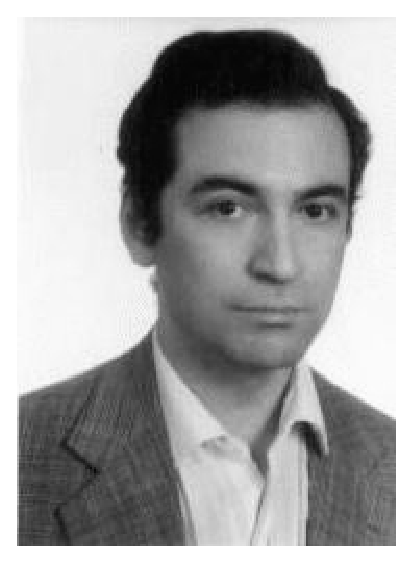
\psfig{file=myfile.eps,height=1.5in,width=1.2in}
\caption{An example of imported eps file.}
\label{f:ex}
\end{center}
\end{figure}
\index{commands!environments!figure}%

It has been generated with the following commands:
\begin{verbatim}
\begin{figure}[htb]
\begin{center}
\ 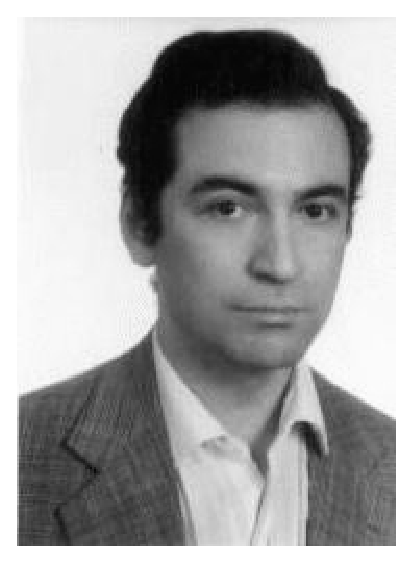
\psfig{file=myfile.eps,height=1.5in,width=1in}
\caption{An example of imported eps file.}
\label{f:ex}
\end{center}
\end{figure}
\end{verbatim}

The command that imports the file is \cn{psfig}, and it also 
controls its size (\texttt{height} and \texttt{width}), and 
can rotate the figure (\texttt{angle}).

Figures can also be drawn by using \LaTeX{} commands. 
Figure \ref{f:circuit} is an example 
(taken from \cite{gms:tlc}).

\begin{figure}[htb]
\begin{center}
   \setlength{\unitlength}{4mm}
   \begin{picture}(12,10)(-2,0)
      \linethickness{0.4pt}
      \qbezier(2.00,6.00)(7.00,6.00)(9.00,3.00)
      \qbezier(2.00,0.00)(7.00,0.00)(9.00,3.00)
      \qbezier(2.00,6.00)(4.00,3.00)(2.00,0.00)
      \qbezier(1.00,6.00)(3.00,3.00)(1.00,0.00)
      \put(9.75,3.00){\circle{1.50}}
      \put(10.50,3.00){\line(1,0){1.50}}
      \put(0.00,5.00){\line(1,0){1.50}}
      \put(0.00,1.00){\line(1,0){1.50}}
   \end{picture}
\caption{An example of picture}
\label{f:circuit}
\end{center}
\end{figure}
\index{picture}%

It has been generated with the following set of commands:
\begin{verbatim}
\begin{figure}[htb]
\begin{center}
   \setlength{\unitlength}{4mm}
   \begin{picture}(12,10)(-2,0)
      \linethickness{0.4pt}
      \qbezier(2.00,6.00)(7.00,6.00)(9.00,3.00)
      \qbezier(2.00,0.00)(7.00,0.00)(9.00,3.00)
      \qbezier(2.00,6.00)(4.00,3.00)(2.00,0.00)
      \qbezier(1.00,6.00)(3.00,3.00)(1.00,0.00)
      \put(9.75,3.00){\circle{1.50}}
      \put(10.50,3.00){\line(1,0){1.50}}
      \put(0.00,5.00){\line(1,0){1.50}}
      \put(0.00,1.00){\line(1,0){1.50}}
   \end{picture}
\caption{An example of picture}
\label{f:cir}
\end{center}
\end{figure}
\end{verbatim}

Those commands have rather obvious meanings. In particular, 
the command \cn{qbezier} 
\index{commands!qbezier@\cn{qbezier}}%
draws a quadratic Bezier curve, 
defined by its two ending points, and a third point (whose 
coordinates are in the middle) that is used as control point. 
Figure \ref{f:qb} illustrates the effect of the control point:

\begin{figure}[htb]
\begin{center}
   \setlength{\unitlength}{.8mm}
   \begin{picture}(55,55)(-15,0)
      \linethickness{1pt}
      \qbezier(0,0)(-10,30)(50,30)
      \qbezier(0,0)(20,50)(50,30)
      \thinlines
      \put(0,0){\line(-1,3){10}}
      \put(50,30){\line(-1,0){60}}
      \put(0,0){\line(2,5){20}}
      \put(50,30){\line(-3,2){30}}
      \put(0,0){\circle*{1}}
      \put(0,-1){\makebox(0,0)[t]{$A_{0,0}$}}
      \put(-10,30){\circle*{1}}
      \put(-10,31){\makebox(0,0)[b]{$B_{10,30}$}}
      \put(50,30){\circle*{1}}
      \put(58,29){\makebox(0,0)[b]{$C_{50,30}$}}
      \put(20,50){\circle*{1}}
      \put(20,51){\makebox(0,0)[b]{$D_{20,50}$}}
   \end{picture}
\caption{Bezier curves}
\label{f:qb}
\end{center}
\end{figure}
\index{Bezier curves}%


That figure has been generated with the following commands:
\begin{verbatim}
\begin{figure}[htb]
\begin{center}
   \setlength{\unitlength}{.8mm}
   \begin{picture}(55,55)(-15,0)
      \linethickness{1pt}
      \qbezier(0,0)(-10,30)(50,30)
      \qbezier(0,0)(20,50)(50,30)
      \thinlines
      \put(0,0){\line(-1,3){10}}
      \put(50,30){\line(-1,0){60}}
      \put(0,0){\line(2,5){20}}
      \put(50,30){\line(-3,2){30}}
      \put(0,0){\circle*{1}}
      \put(0,-1){\makebox(0,0)[t]{$A_{0,0}$}}
      \put(-10,30){\circle*{1}}
      \put(-10,31){\makebox(0,0)[b]{$B_{10,30}$}}
      \put(50,30){\circle*{1}}
      \put(58,29){\makebox(0,0)[b]{$C_{50,30}$}}
      \put(20,50){\circle*{1}}
      \put(20,51){\makebox(0,0)[b]{$D_{20,50}$}}
   \end{picture}
\caption{Bezier curves}
\label{f:qb}
\end{center}
\end{figure}
\end{verbatim}


\chapter{An example of Mathematical writing}
\index{An example of Mathematical writing%
@\emph{An example of Mathematical writing}}%

\section{Generalized Fatou's Lemma}
\index{Generalized Fatou's Lemma%
@\emph{Generalized Fatou's Lemma}}%

Here we show an application of the following lemma:

\begin{lem}[Generalized Fatou's Lemma] \label{l:fatou}

Let $A$ be a Dedekind ring and $F$ a rational series 
in $A[[X]]$, i.e., $F = p/q$ for some 
$p, q \in A[X]$. Then there exist two polynomials 
$P, Q \in A[X]$ such that $F = P/Q$, 
where $P$ and $Q$ are relatively prime and 
$Q(0) = 1$.

\end{lem}

\proof
See \cite{bertin:psn}, p.~15, theorem~1.3.
\endproof

\begin{thm} \label{l:req}
Let $\{c_n\}_{n=-\infty}^{\infty}$ a set of 
elements from $K$ such that $c_n \in k'$ for every 
$n \geq n_0$, and verifying the following recurrence 
relation of order M:
\begin{equation}
c_n\ =\ r_1\,c_{n-1} + r_2\,c_{n-2} + \dots + r_M\,c_{n-M}
\end{equation}
for every $n \in \mathbb Z$, where $r_1,r_2,\dots,r_M$ are in 
$K$, $r_M \neq 0$. 
Then:

\item{(i)} The coefficients $r_1,r_2,\dots,r_M$ are in 
$k'$, and for every $n \in \mathbb Z$, $c_n \in k'$.

\item{(ii)} If $c_n \in \mathcal O_{k',v}$ 
for every $n \geq n_0$, then the coefficients 
$r_1,r_2,\dots,r_M$ are all in 
$\mathcal O_{k',v}$.

\end{thm}


\proof 

\item{(i)} Let $C_n$ and $R$ be the matrices:

\begin{equation}
C_n\ =
\ \left(
\begin{array}{llll}
              c_n & c_{n+1} & \hdots & c_{n+M-1} \\
              c_{n+1} & c_{n+2} & \hdots  & c_{n+M} \\
              \vdots & \vdots & \ddots & \vdots \\
              c_{n+M-1} & c_{n+M} & \hdots & c_{n+2M-2}
\end{array}
\right)
\end{equation}
and
\begin{equation}
R\ =
\ \left(
\begin{array}{lllll}
              0 & 1 & 0 & \hdots & 0 \\
              0 & 0 & 1 & \hdots & 0 \\
             \vdots & \vdots & \vdots & \ddots & \vdots \\
              0 & 0 & 0 & \hdots & 1 \\
              r_M & r_{M-1} & r_{M-2} & \hdots & r_1 
\end{array}
\right)
\end{equation} 

We have that $C_{n+1} = R\,C_n$. Since the recurrence 
relation is of order M, $C_n$ is non singular. 
On the other hand, $R = C_{n+1}\,C_{n}^{-1}$. Since the 
elements of $C_n$ are in $k'$ for $n \geq n_0$, the entries 
of $R$, and those of $R^{-1}$, will be in $k'$. Since 
$C_{n-1} = R^{-1}\,C_n$, we get that the entries of 
$C_n$ will be in $k'$ also for $n < n_0$. 

\item{(ii)} For each $t \geq n_0$ define the formal 
power series 

\begin{equation}
F_t(X)\ =\ \sum_{n=0}^{\infty} c_{t+n}\,X^n
\end{equation}
which is in $\mathcal O_{k',v}[[X]]$. 
We have $F_t(X) = p_t(X)/q(X)$, 
where $p_t(X),q(X) \in k'[X]$ are the following:
\begin{equation}
p_t(X)\ =\ \sum_{j=0}^{M-1} \Bigl( c_{t+j} - 
                    \sum_{i=1}^{j} r_i\,c_{t+j-i} \Bigr)\,X^j
\end{equation}
\begin{equation}
q(X)\ =\ 1 - r_1\,X - r_2\,X^2 - \dots - r_M\,X^M
\end{equation}
This can be checked by multiplying $F_t(X)$ by $q_t(X)$ 
and using the recurrence relation, which gives 
$F_t(X)\,q(X) = p_t(X)$ (see \cite{poorten:sp}). 

Now we will prove that $p_t(X)$ and $q(X)$ are relatively 
prime. To do so, we will see that they cannot have any 
common root (in $\overline {k'}$). In fact, assume 
that $\alpha$ is a common root of $p_{t_0}(X)$ and $q(X)$ 
for some $t_0 \geq n_0$, i.e.: 
$p_{t_0}(\alpha) = q(\alpha) = 0$. 
Since $q(0)=1$, then $\alpha \neq 0$. Now we have:
\begin{equation}
X\,F_{t_0+1}(X) = F_{t_0}(X) - c_{t_0}
\end{equation}
so:
\begin{multline}
X\,p_{t_0+1}(X) = X\,q(X)\,F_{t_0+1}(X) \\
= q(X)\,(F_{t_0}(X) - c_{t_0}) = p_{t_0}(X) - c_{t_0}\,q(X)
\end{multline}
Hence $p_{t_0+1}(\alpha) = 0$, which means that $\alpha$ is 
also a root of $p_{t_0+1}(X)$. By induction we get that 
$p_t(\alpha) = 0$ for every $t \geq t_0$. Grouping the 
terms of $p_t(X)$ with respect to $c_t,c_{t+1},\dots,c_{t+M-1}$, 
we get:
\begin{equation}
p_t(X) = \sum_{j=0}^{M-1} a_j(X)\,c_{t+j}
\end{equation}
where 
\begin{equation}
a_j(X) = X^j\,\Bigl( 1 - \sum_{i=1}^{M-j-1} r_i\,X^i \Bigr)
\end{equation}
Note that $a_0(X),a_1(X),\dots,a_{M-1}(X)$ do not depend on t. 
On the other hand $p_t(\alpha)=0$ implies
\begin{equation}
\label{e:coldep}
\sum_{j=0}^{M-1} a_j(\alpha)\,c_{t+j} = 0
\end{equation}
for every $t \geq t_0$. Note that $a_{M-1}(\alpha)=\alpha^{M-1}
\neq 0$, so $a_0(\alpha),a_1(\alpha),\dots,a_{M-1}(\alpha)$ 
are not all zero, and (\ref{e:coldep}) means that the columns 
of the matrix $C_{t_0}$ are linearly dependent, so 
$\det C_{t_0}=0$, which contradicts the fact that $C_{t_0}$ 
is non singular. Hence, the hypothesis that $p_t(X)$ and 
$q(X)$ have a common root has to be false. This proves that 
$p_t(X)$ and $q(X)$ are relatively prime. 

By (generalized Fatou's) lemma~\ref{l:fatou}, 
and taking into account that 
$\mathcal O_{k',v}$ is a Dedekind ring, 
we get that there exist two relatively prime 
polynomials $P_t(X)$ and $Q_t(X)$ in 
$\mathcal O_{k',v}[X]$ such that 
$F_t(X) = P_t(X)/Q_t(X)$ and $Q_t(0)=1$. Hence: 
$p_t(X)\,Q_t(X) = q(X)\,P_t(X)$. By unique factorization 
of polynomials in $k'[X]$, there is a $u \in k'$ such that 
$P_t(X) = u\,p_t(X)$ and $Q_t(X) = u\,q_t(X)$. Since 
$Q_t(0)=q(0)=1$, we get that $u=1$, so 
$P_t(X) = p_t(X)$ and $Q_t(X) = q(X)$. 
Hence, the coefficients of $q(X)$ are in 
$\mathcal O_{k',v}$. 

\endproof


\section{Other examples of Mathematical writing}

\subsection{An example of commutative diagram}
\index{An example of commutative diagram%
@{An example of commutative diagram}}%

The following is an example of commutative diagram.
\index{commutative diagram}%
It requires the \texttt{amscd} package.
\index{amscd package@{\texttt{amscd} package}}

\begin{equation*}
\newcommand{\End}{\operatorname{End}}
\begin{CD}
S^{{\mathcal{W}}_\Lambda}\otimes T   @>j>>   T\\
@VVV                                    @VV{\End P}V\\
(S\otimes T)/I                  @=      (Z\otimes T)/J
\end{CD}
\end{equation*}

That diagram has been made with the following commands:

\begin{verbatim}
\newcommand{\End}{\operatorname{End}}
\begin{CD}
S^{{\mathcal{W}}_\Lambda}\otimes T   @>j>>   T\\
@VVV                                    @VV{\End P}V\\
(S\otimes T)/I                  @=      (Z\otimes T)/J
\end{CD}
\end{verbatim}

\subsection{Using AMS fonts}
\index{Using AMS fonts@{Using AMS fonts}}

To use AMS fonts it is necessary to choose from an assortment 
of \LaTeX{} packages. For instance the command 
\cn{usepackage\{amsfonts\}} calls in the \emph{amsfonts} package, 
which provides blackboard bold letters (e.g. $\mathbb{R}$) and 
some math symbols. A superset of that package is 
\emph{amssymb}. Other packages are \emph{eufrak} 
for Frankfurt letters (e.g. $\mathfrak{R}$)
and \emph{eucal} for Euler script 
(e.g. $\mathcal{R}$). 
Consult the \LaTeX{} documentation about this subject 
for additional information.





% Appendix


                 % Here I use single spacing for the Appendix
\baselineskip=15.5pt plus .5pt minus .2pt

                 % Use this for one and a half spacing
% \baselineskip=20.5pt plus .5pt minus .2pt 

                 % This is double spacing. Since it is the 
                 % default, it is unlikely that it will 
                 % ever needed. Included just in case. 
% \baselineskip=23.5pt plus .5pt minus .2pt

\appendix
\index{Appendix@\emph{Appendix}}%

The source \LaTeX{} file for this document.

Here is the full source of this file. Look near its 
end if you are curious about how a \LaTeX{} file can 
include its own source.

\vfill

\verbatiminput{\jobname}  % Command to include the source
                              % of this document.

% Index

\printindex%    % Include the index here.


\nocite{*}      % This command causes all items in the 
                % bibliographic database to be added to 
                % the bibliography, even if they are not 
                % explicitly cited in the text. 


\bibliographystyle{plain}  % Here the bibliography 
\bibliography{diss}        % is inserted.
\index{Bibliography@\emph{Bibliography}}%

% Vita page %

\begin{vita}
\index{Vita@\emph{Vita}}%

Miguel A. Lerma 
\index{Miguel A. Lerma}%
was born in Madrid, Spain, on March 31, 1954, 
the son of Miguel Lerma and Pilar Usero. After completing his 
High School studies in Madrid, Spain, in 1971, he entered 
the Universidad Complutense in Madrid. 
He received degree of Licenciado (B.\,S.) in Physics 
from the Universidad Complutense in 1977, 
and in Mathematics from the same university in 1978. 
The next year he got a Lecturer 
position for one year at the department of Mathematics 
in the Universidad Complutense, and a tenured position 
as a Math Teacher in High School. In 1989 he started 
graduate studies in the department of Computer Science 
of the Universidad Polit\'ecnica in Madrid. The next year 
he got a position as an untenured 
Assistant Professor in the Department of Computer Science 
of the Universidad Polit\'ecnica, where he remained until 
1993. In 1991 he received a Doctor (Ph.\,D.) degree 
in Computer Science. In September 1993, he entered 
the Graduate School of the University of Texas at Austin.

\end{vita}


\end{document}
